\begin{figure}[!h] 
\centering 
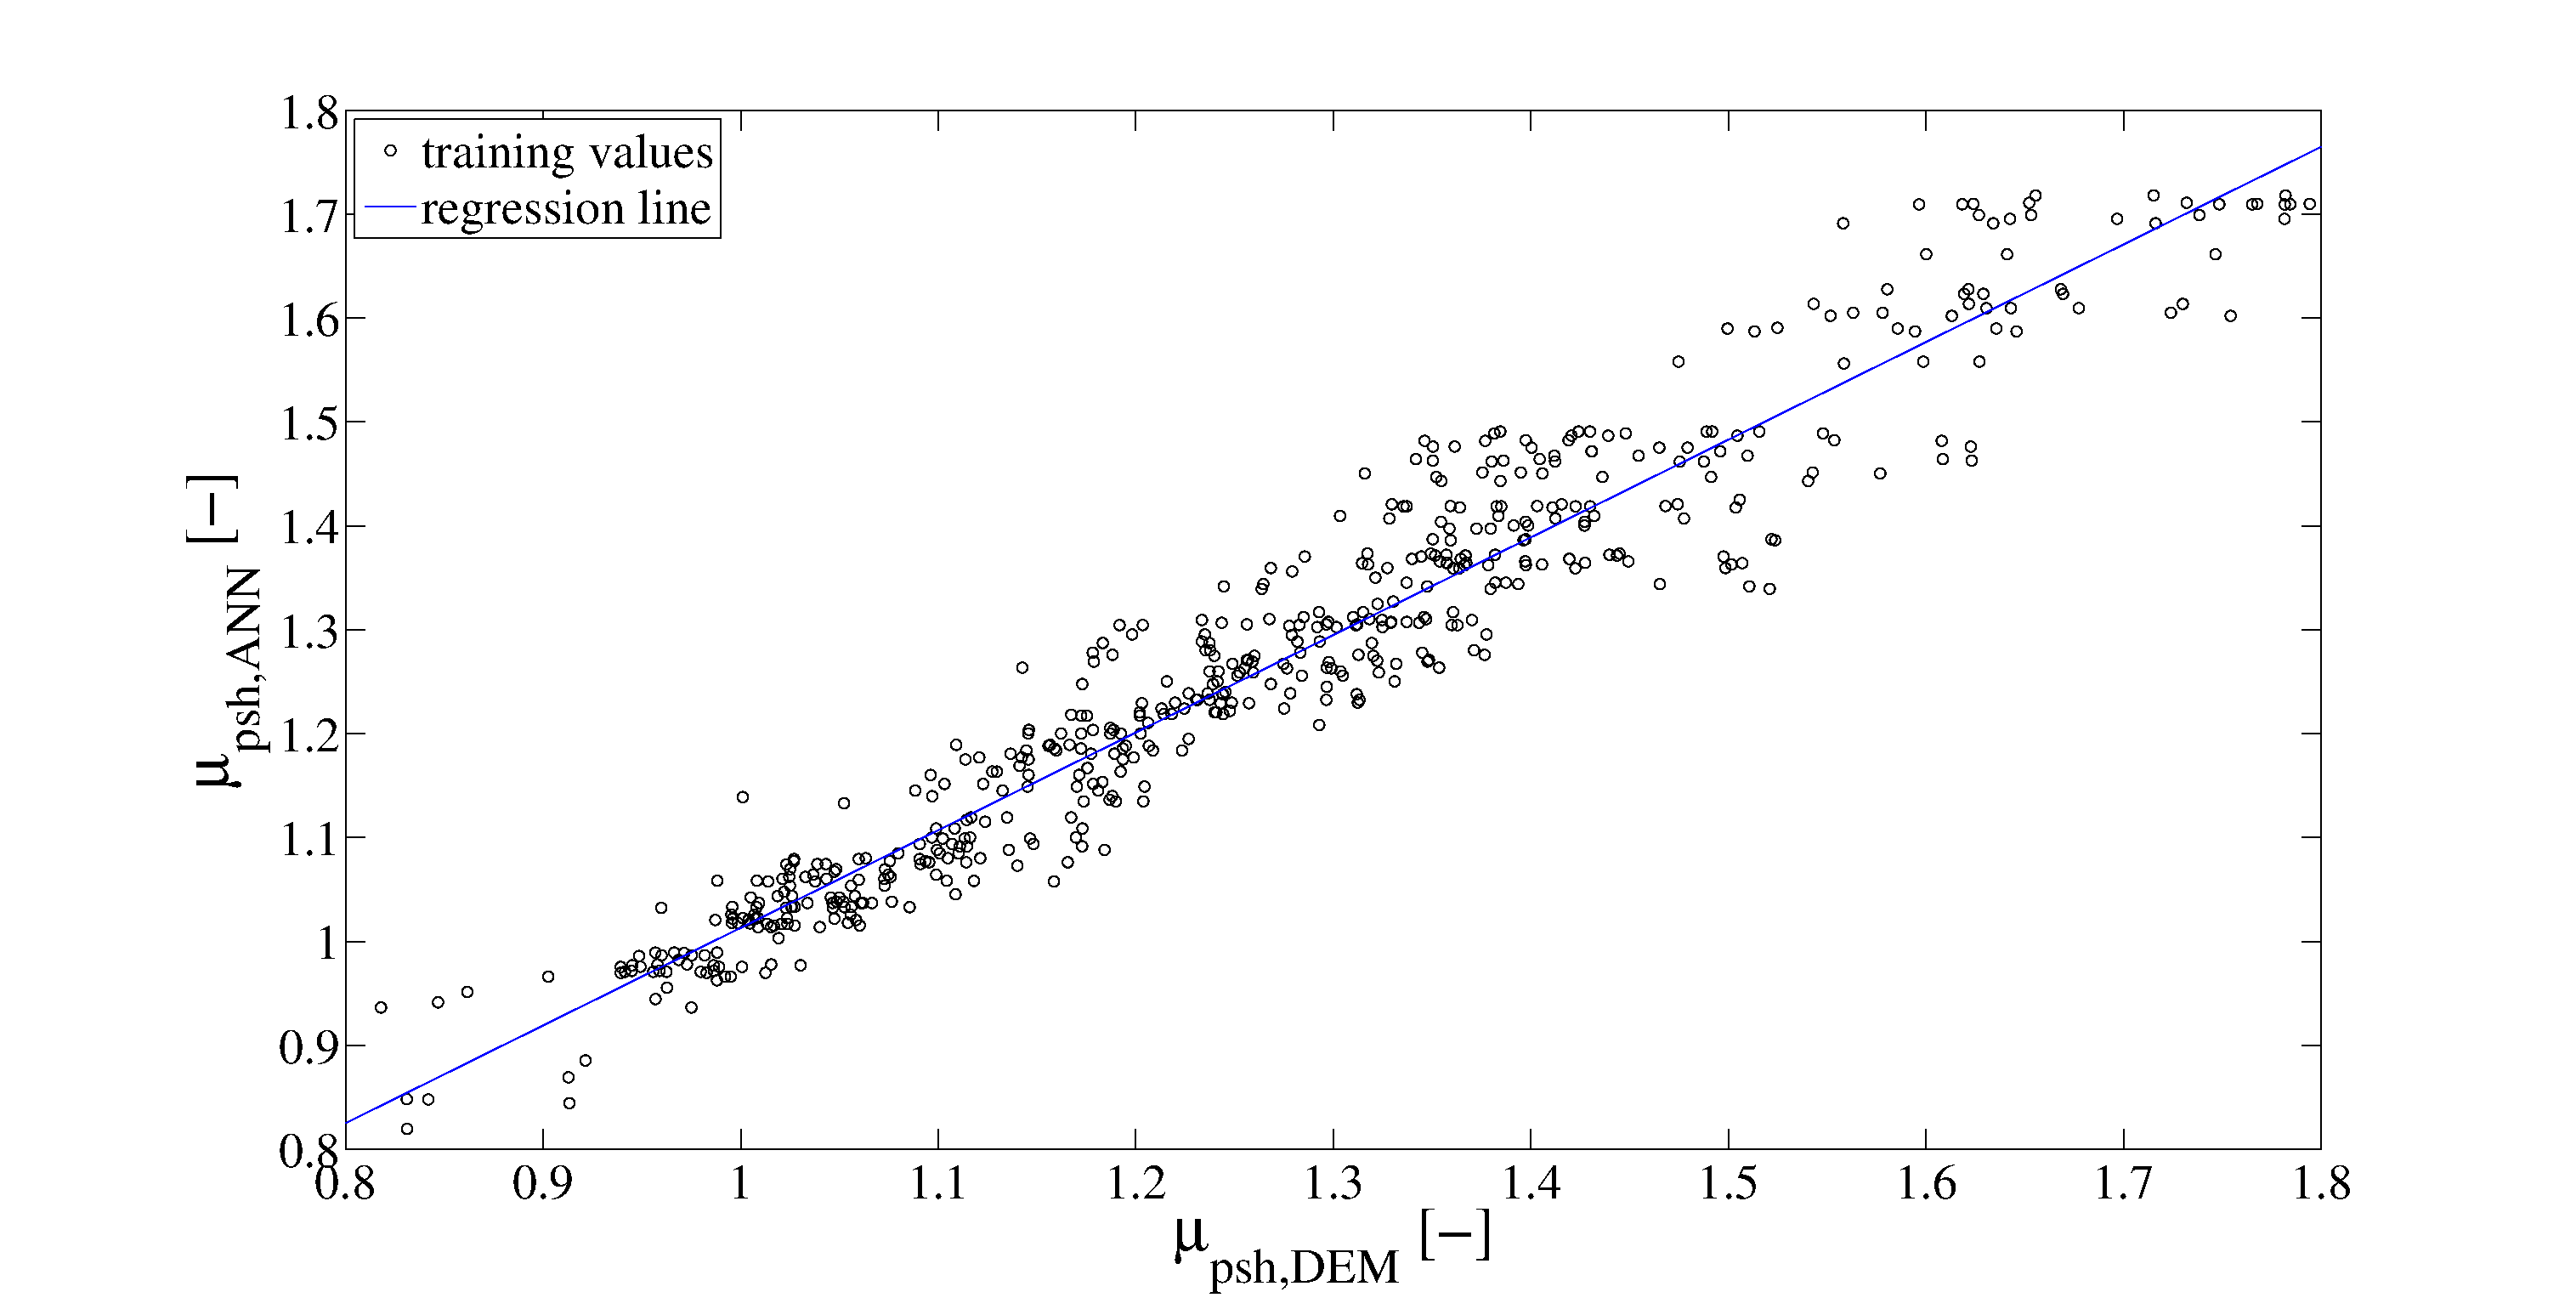
\includegraphics[width=.96\textwidth]{images/original/22regression}
%[width=.96\textwidth]
\caption[Comparison between prediction of the trained NN and full DEM
simulation]{Comparison between prediction of the trained Neural Network ($NN$)
and 546 full DEM simulations of the coefficient of pre-shear ($\mu_{psh}$). In
this case the regression line is nearly linear, and demonstrates the accurate
prediction of the $NN$.}
\label{fig:22regression} 
\end{figure}

% Regression plot - $\mu_{psh}$. In this case the
% $Output = 0.96 \cdot Target + 0.046$. With 546 simulations the $R^2 = 0.98044$. The plot
% presents a consistent agreement between the $DEM$ results distribution and the $NN$ regression line.
% \begin{figure}[htp]
%     \centering
%     
\includegraphics[width=.2\textwidth]{images/vitae/lbenvenuti}
%     \caption{OpenMP, MPI, MPI/OpenMP Hybrid runs of Box in a box testcase on 32
%     cores. The OpenMP-only run suffers from limited memory bandwidth in
%     memory-bound algorithms inside of the Modify section of the code. MPI-only has
%     low averaged runtimes for each section, but a very large Other timing, which
%     hints for a large amount of load-imbalance. Hybrid timings are a bit worse
%     on average, but because of better balancing, processes have lower wait times
%     inside of Other timing.}
% 	\label{fig:boxInBoxComparison}
